% !TEX encoding = UTF-8 Unicode
\documentclass[a4paper]{article}

\usepackage{color}
\usepackage{url}
\usepackage[T2A]{fontenc} % enable Cyrillic fonts
\usepackage[utf8]{inputenc} % make weird characters work
\usepackage{graphicx}
\usepackage{multirow}
\usepackage[english,serbian]{babel}
\usepackage[most]{tcolorbox}
%\usepackage[english,serbianc]{babel} %ukljuciti babel sa ovim opcijama, umesto gornjim, ukoliko se koristi cirilica

\usepackage[unicode]{hyperref}
\hypersetup{colorlinks,citecolor=green,filecolor=green,linkcolor=blue,urlcolor=blue}
\usepackage{mathtools}
\usepackage{listings}
\usepackage{multirow}
\usepackage{todonotes}
\newcommand\todos[1]{\textcolor{red}{#1}}

%\newtheorem{primer}{Пример}[section] %ćirilični primer
\newtheorem{primer}{Primer}[section]

\definecolor{mygreen}{rgb}{0,0.6,0}
\definecolor{mygray}{rgb}{0.5,0.5,0.5}
\definecolor{mymauve}{rgb}{0.58,0,0.82}

\lstset{ 
  backgroundcolor=\color{white},   % choose the background color; you must add \usepackage{color} or \usepackage{xcolor}; should come as last argument
  basicstyle=\footnotesize,        % the size of the fonts that are used for the code
  breakatwhitespace=false,         % sets if automatic breaks should only happen at whitespace
  breaklines=true,                 % sets automatic line breaking
  captionpos=b,                    % sets the caption-position to bottom
  commentstyle=\color{mygreen},    % comment style
  deletekeywords={...},            % if you want to delete keywords from the given language
  escapeinside={\%*}{*)},          % if you want to add LaTeX within your code
  extendedchars=true,              % lets you use non-ASCII characters; for 8-bits encodings only, does not work with UTF-8
  firstnumber=1000,                % start line enumeration with line 1000
  frame=single,	                   % adds a frame around the code
  keepspaces=true,                 % keeps spaces in text, useful for keeping indentation of code (possibly needs columns=flexible)
  keywordstyle=\color{blue},       % keyword style
  language=Python,                 % the language of the code
  morekeywords={*,...},            % if you want to add more keywords to the set
  numbers=left,                    % where to put the line-numbers; possible values are (none, left, right)
  numbersep=5pt,                   % how far the line-numbers are from the code
  numberstyle=\tiny\color{mygray}, % the style that is used for the line-numbers
  rulecolor=\color{black},         % if not set, the frame-color may be changed on line-breaks within not-black text (e.g. comments (green here))
  showspaces=false,                % show spaces everywhere adding particular underscores; it overrides 'showstringspaces'
  showstringspaces=false,          % underline spaces within strings only
  showtabs=false,                  % show tabs within strings adding particular underscores
  stepnumber=2,                    % the step between two line-numbers. If it's 1, each line will be numbered
  stringstyle=\color{mymauve},     % string literal style
  tabsize=2,	                   % sets default tabsize to 2 spaces
  title=\lstname                   % show the filename of files included with \lstinputlisting; also try caption instead of title
}

\begin{document}

\title{Hibrid neuronske mreže, genetskog algoritma i reinforcement learninga za igranje top-down shooter igre\\~\\ \small{Seminarski rad u okviru kursa\\Računarska inteligencija\\ Matematički fakultet}}
\author{Đaković Branko, Filip Kristić, Krčmarević Mladen\\brankodjakovic08@gmail.com, filip.kristic96@gmail.com\\ mladenk@twodesperados.com}

%\date{9.~april 2015.}
\maketitle

\abstract{ U radu će biti prikazana upotreba “reinforcement learing”-a i genetskog algoritma za generisanje težina neuronske mreže koja igra top-down shooter igru “Shrodinger's shooter”. Ovaj pristup spada u Neuro-evoluciju\cite{neuroevolution}, s tim što se menjaju samo težine neruonske mreže dok je struktura fiksna. Za pisanje kodova je korišćen programski jezik C++ i biblioteka FANN sa omotačem za C++. Daćemo kratak opis igre kao i dva rešenja koja se razlikuju po načinu reprezentacije ulaza za neuronsku mrežu.
} 
\tableofcontents

\newpage

\section{Uvod}
\label{sec:uvod}
\par “Shrodinger's shooter” je shooter igra koju smo razvili za predmet Razvoj softvera u kojoj je cilj igrača da što duže preživi nalete protivnika. Igrica koristi 2D fiziku uz 3D grafiku, a mapa je kvadratnog oblika i sadrži zidove. Moguće akcije igrača su: “idi gore”, “dole”, “levo”, “desno” kao i dijagonalno kretanje njihovom kombinacijom, podešavanje pozicije nišana, repetiranje oružja i pucanje. Zbog kompleksnosti su izbačeni prva pomoć, pancir, granate i različito oružje. Cilj neuronske mreže\cite{neural} je da na osnovu trenutne situacije igrača da njegovu sledeću akciju. 
%%%%%
\begin{figure}[h!]
	\begin{center}
		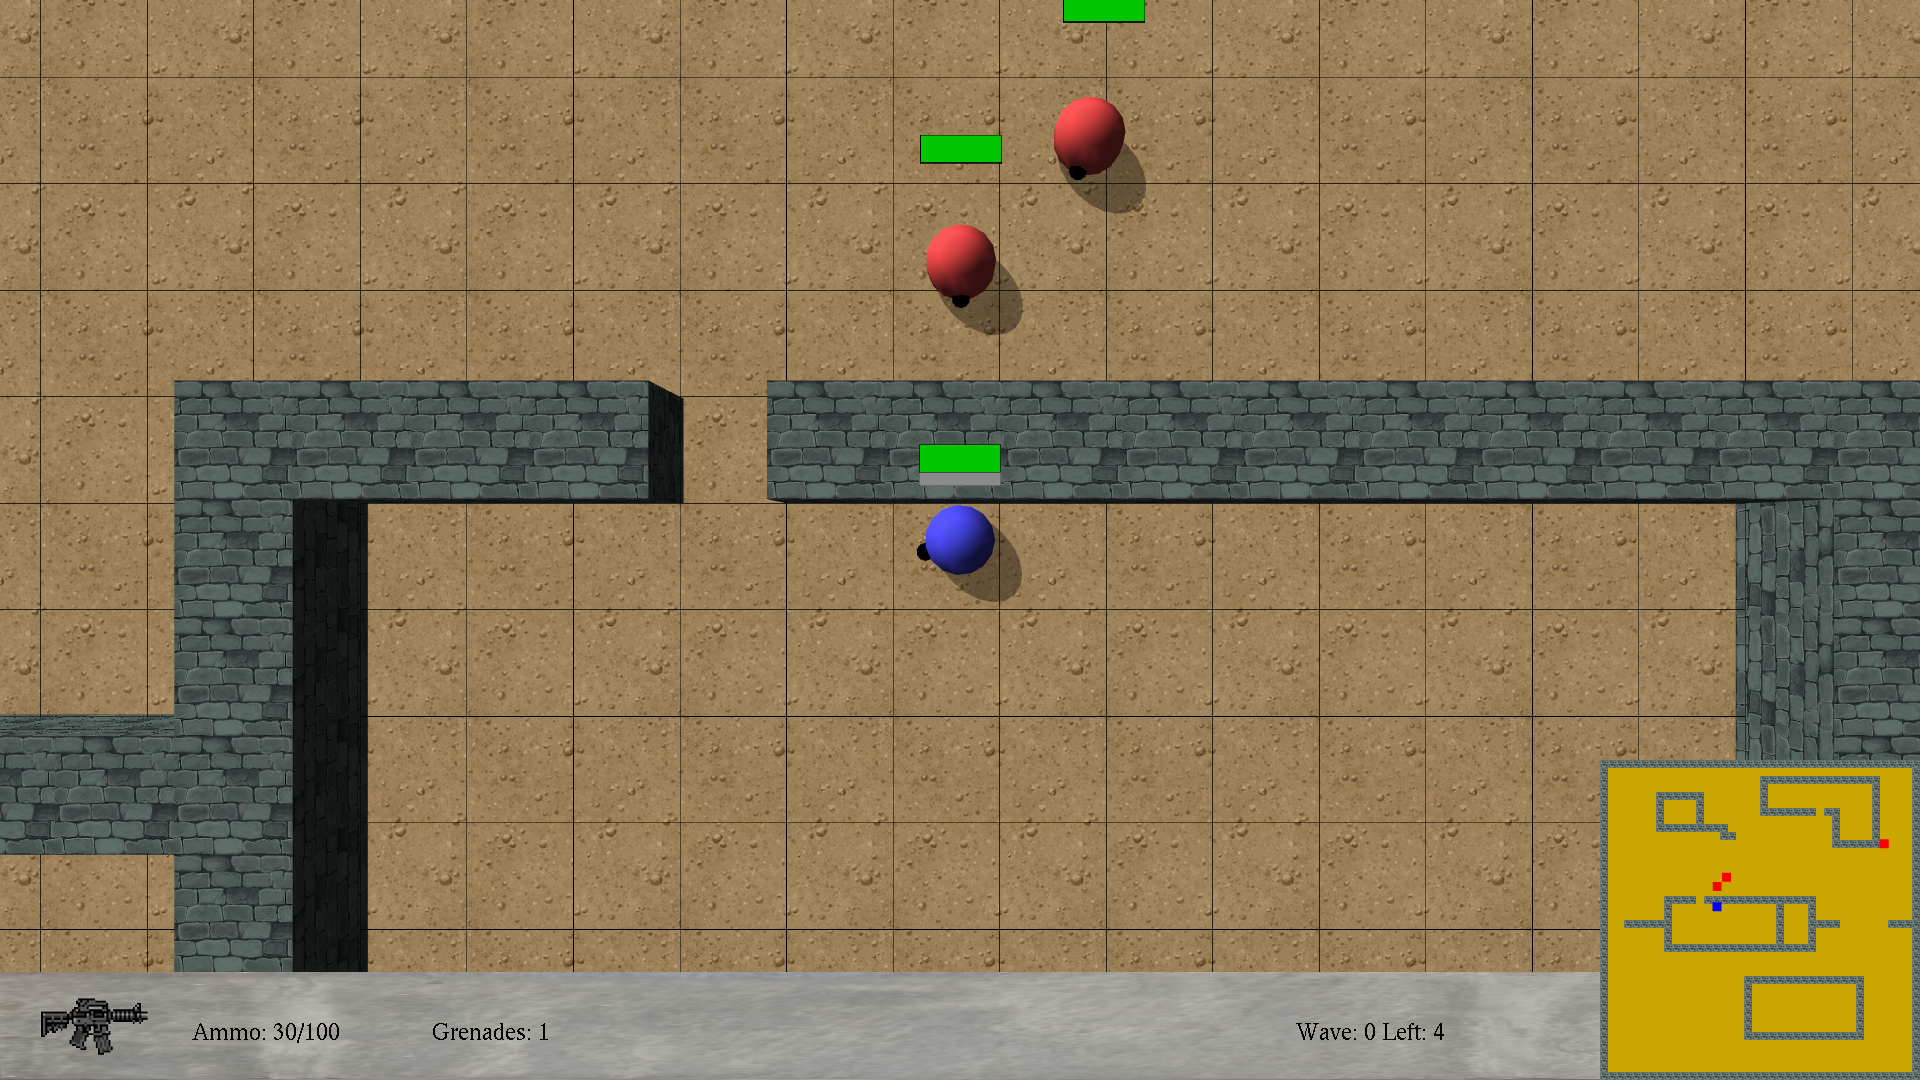
\includegraphics[scale=0.18]{igra.png}
	\end{center}
	\caption{Schrodinger's shooter}
	\label{fig:igra}
\end{figure}
  

\section{Opis rešenja}
\label{sec:opisResenja}
\par Program ima tri načina izvršavanja:
\begin{tcolorbox}
./Schshooter.out
\end{tcolorbox}
koji obuhvata učitavanje rešenja u vidu neuronske mreže i igranje igrice uz grafički prikaz,
\begin{tcolorbox}
./Schshooter.out -t brojIteracija
\end{tcolorbox}
koji vrši treniranje sa brojem iteracija “brojIteracija” bez grafičkog prikaza i
\begin{tcolorbox}
./Schshooter.out -tv brojIteracija
\end{tcolorbox}
koji vrši treniranje sa brojem iteracija “brojIteracija”  sa grafičkim prikazom.

\newpage
\par Trening započinje kreiranjem početne generacije genetskog algoritma\cite{genetic} (slika \ref{fig:genetic}.\footnote{Slika preuzeta sa: \url{https://apacheignite.readme.io/docs/genetic-algorithms}}) kod koje svaki hromozom ima prilagođenost (fitness) jednak nuli. Hromozomi su predstavljeni sadržajem tj. nizom brojeva u pokretnom zarezu koji predstavlja težine svih veza mreže i jednim brojem u pokretnom zarezu koji predstavlja prilagođenost tog hromozoma. Težine se uzimaju nasumično iz intervala [-10, 10] koji je takođe nasumično izabran. Broj hromozoma u generaciji kao i broj generacija u oba rešenja iznose po nekoliko stotina. O ulazu će više biti rečeno u narednom poglavlju.

\begin{figure}[h!]
	\begin{center}
		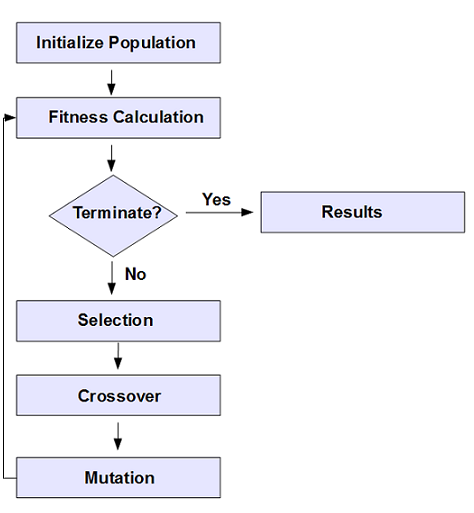
\includegraphics[scale=0.7]{genetic.png}
	\end{center}
	\caption{Genetski algoritam}
	\label{fig:genetic}
\end{figure}

\par Nakon kreiranja generacije redom se uzimaju hromozomi i težine veza neuronske mreže se postavljaju na sadržaj hromozoma. Veličina ulaznog sloja u prvom rešenju je 191, a 10 u drugom. oba rešenja imaju samo jedan skriven sloj koji je veličine 10 u prvom zbog ogromnog broja veza usled veličine ulaza i 8 u drugom. Za aktivacionu funkciju je korišćena linearna aproksimacija sigmoidne funkcije. Sigmoidna funkcija je oblika: \footnote{Preuzeto iz dokumentacije fann biblioteke. \url{http://leenissen.dk/fann/html/files/fann_cpp-h.html}}
\begin{tcolorbox}
\begin{center}
x - ulaz \\
y - izlaz \\ 
s - nagib i \\
d - derivacija \\
raspon: 0 < y < 1 \\
\end{center}
\begin{equation}
y = \frac{1}{1 + \mathrm{e}^{-2 \times s \times x}}
\end{equation}
\begin{equation}
d = 2 \times s \times y \times (1 - y)
\end{equation}
\end{tcolorbox}
\noindent  Stopa učenja nije podešena pošto nema nikakvog uticaja na dati problem. Izlazni sloj sadrži pet neurona čiji izlazi imaju vrednosti u intervalu [0,1] a koji regulišu kretanje gore-dole, levo-desno, treći ugao pod kojim igrač nišani,da li da puca i da li da dopuni municiju. Prva dva izlaza su podeljena u tri intervala [0,0.33], (0.33-0.66] i (0.66-1] koji redom odgovaraju kretanju gore (levo), bez kretanja i dole (desno). Treći izlaz se skalira na [-$\pi$, $\pi$] i ugao igrača se postavlja na datu vrednost a četvrti i peti daju potvrdan odgovor za vrednosti manje od 0.5, a negativan u suprotnom. U svakoj iteraciji programa se ažuriraju pozicija i akcije igrača u zavisnosti od izlaza mreže. “Reinforcement learing” se koristi prilikom izračunavanja prilagođenosti svakog hromozoma tako što za svaku dobru akciju u vidu eliminacija ili nanošenja štete hromozom dobija nagradu u vidu poena. Prilagođenost se računa na osnovu naredne formule, a najbolje ocenjen hromozom se čuva. U drugom rešenju je dodatno implementirano višestruko izvršavanje za svaki hromozom, a zatim uzimanje srednje vrednosti dobijenih prilagođenosti.
\begin{tcolorbox}
fintess = eliminacije * 50 + šteta * 0.5
\end{tcolorbox}

\subsection{Selekcija, ukrštanje i mutacija}
\par Po obradi svih hromozoma generacije, ukoliko ima još iteracija, vrši se selekcija hromozoma koji će učestvovati u izradi nove generacije. Selekcija se vrši ruletskim pristupom, tako što se računa zbir prilagođenosti svih hromzoma i svaki ima šansu da bude izabran srazmerno odnosu njegove i celokupne prilagođenosti. Nakon izbora hromozoma koji učestvuju u reprodukciji nasumično se biraju dva roditelja i vrše se ukrštanje i mutacija koji su implementirani na različite načine u prvom i drugom rešenju. Svaki par roditelja kreira dva deteta i to se vrši sve dok ne bude ispunjena nova populacija. 
\begin{tcolorbox}
\begin{center}
Ukrštanje u prvom rešenju: \\
\end{center}
i - nasumičan broj od 0 do veličine sadržaja hromozoma;\\
dete1 = sadržaj roditelja1 do i + sadržaj roditelja2 od i do kraja; \\
dete2 = sadržaj roditelja2 do i + sadržaj roditelja1 od  i do kraja; \\
\begin{center}
Mutacija u prvom rešenju:  \\
\end{center}
t - nasumičan broj u pokretnom zarezu iz intervala [0,1];\\
Ukoliko je t manje od stope mutacije: \\
\hphantom{tcolorbox}Promeniti nasumičan element sadržaja hromozoma;
\end{tcolorbox}

\begin{tcolorbox}
\begin{center}
Ukrštanje u drugom rešenju: \\
\end{center}
Za svaki element i sadržaja hromozoma uraditi:\\
\hphantom{tcolorbox}t - nasumičan broj u pokretnom zarezu iz intervala [0,1];\\
\hphantom{tcolorbox}Ako je t < 0.5: \\
\hphantom{tcolorbox}\hphantom{tcolorbox}dete1[i] = roditelj1[i]; \\
\hphantom{tcolorbox}\hphantom{tcolorbox}dete2[i] = roditelj2[i]; \\
\hphantom{tcolorbox}Inače: \\
\hphantom{tcolorbox}\hphantom{tcolorbox}dete1[i] =  roditelj2[i]; \\
\hphantom{tcolorbox}\hphantom{tcolorbox}dete2[i] =  roditelj1[i]; \\
\begin{center}
Mutacija u drugom rešenju:  \\
\end{center}
Za svaki element i sadržaja hromozoma uradi:\\
\hphantom{tcolorbox}t - nasumičan broj u pokretnom zarezu iz intervala [0,1];\\
\hphantom{tcolorbox}Ukoliko je t manje od stope mutacije: \\
\hphantom{tcolorbox}\hphantom{tcolorbox}Promeniti i-ti element sadržaja hromozoma;
\end{tcolorbox}

\par Celokupan navedeni postupak se zatim ponavlja dok nije zadovoljen kriterijum zaustavljanja, tj. dok se ne premaši zadati broj iteracija. Najbolja jednika kao i svi hromozomi poslednje generacije se čuvaju u vidu neuronskih mreža u tekstualnim datotekama radi čuvanja progresa i nastavka treniranja.

\section{Upoređivanje rešenja}
\label{sec:uporedjivanjeResenja}

\par U ovom poglavlju biće opisana dva eksperimentalna rešenja problema. Njihova suštinska razlika je način na koji je predstavljen ulaz neuralne mreze igrača, tj. način na koji se opisuje trenutno stanje okoline igrača.
\subsection {Prvo rešenje}
\par U prvom rešenju pokušali smo sa pristupom predstavljanja celokupne okoline igrača, naime svako polje na ekranu predstavlja jedan ulazni čvor koji može imati vrednosti: 0 ako je polje prazno, -1 ako se na njemu nalazi protivnički igrač i 1 ako je u pitanju zid. Ovaj unos je poprilično velik jer na ekranu, u datom trenutku, igrač može da vidi 190 polja, te se to preslikava u 190 ulaznih čvorova i još jedan za količinu trenutne municije.  Igrač se uvek nalazi na polju (5, 9), tj. u sredini mape koja je na primeru obeleženma sa  “P” radi preglednosti, a prilikom izvršavanja je 0.  
\newline
\begin{tcolorbox}
\begin {center}
1000000000000000000 \\
1000000000000000000\\
1000000000000000000\\
1000000011110111111\\
1000000010000000-100\\
100000001P000000000\\
10000000000-10000000\\
1000000010000000000\\
1000000010000000000\\
1000000011111111111\\
\end{center}
\end{tcolorbox}

Trening je vršen na populaciji od 300 jedinki po generaciji u 300 iteracija.
\newline
\begin{tcolorbox}
\begin {center}
Karakteristike hardvera na kome je vršen trening: \\
\end {center}
CPU: intel-i5 2500k \\
GPU: AMD Radeon 6850 \\
RAM: 4GB DDR3 \\
OS: Ubuntu 16.04 \\
\end{tcolorbox}
\noindent Vreme trajanja je oko 10h posle čega je dobijena konfiguracija koja nije davala dobre rezultate. Zaključeno je da ovaj pristup suštinski ne konvergira ka dobrom rešenju te je primenjen drugi pristup sa drastično smanjenjim ulazom neuralne mreze.

\subsection {Drugo rešenje}
\par U drugom rešenju znatno je smanjen broj ulaznih čvorova. Prvi ulaz je ugao prema najblizem vidljivom protivniku, a drugi trenutna kolicina municije. Okolina je predstavljena preko senzora. Postoji 8 senzora, po jedan u svakom pravcu od igrača (gore, dole, levo, desno i dijagonale).  Senzori proveravaju broj praznih mesta u svojim pravcima,  postavljaju se na određen broj i skaliraju na interval [0, 1] u odnosu na ukupan broj polja do kraja ekrana. 

Ocekivano je da ce ovaj pristup dati smislenije rezultate zbog drastično manje kolicine ulaznih podataka. Uprkos smanjenom ulazu su dobijeni slični rezultati kao kod prvog rešenja, tj. igrači koji se nasumično kreću i pucaju.

Trening za ovaj pristup vršen je na populaciji od 100 jedinki po generaciji u 300 iteracija, s tim što se za svaku jedinku fitnes računao po pet puta pa je uzeta srednja vrednost.
\newline
\begin{tcolorbox}
\begin {center}
Karakteristike hardvera na kome je vršen trening: \\
\end {center}
CPU: intel-i5 7300hq \\
GPU: NVIDIA GeForce 1060 \\
RAM: 16GB DDR4 \\
OS: Windows Subsystem for Linux - Ubuntu 18.04 \\
\end{tcolorbox}


 \newpage
\section{Zaključak}
\label{sec:zakljucak}

\par Tema ovog rada bila je da se prikaže upotreba tehnika “reinforcement learing”-a,  neuronskih mreza i genetskog algoritma u svrhu igranja kompjuterskih igrica tj konkretno igrice “Shrodinger's shooter”. Postoji više načina na koji moze da se realizuje “računarski igrač”,  predstavljeni pristup nije dao dobre rezultate. Podešavanjem parametara i načina predstavljanja unosnih podataka, kao i različitim dužinama treninga pokusano je da se sistem navede na bolja rešenja ali idalje nije dobijeno zadovoljavajuće ponašanje. Analizom dobijenih rezultata zaključujemo da za dati problem nije dovoljno samo menjanje težine i da bi se, za ovaj konkretan problem, verovatnije dobili bolji rezultati primenom neke druge metode poput NEAT\cite{neat}  Algoritma gde se menja cela struktura neuronske mreze u procesu učenja.


\addcontentsline{toc}{section}{Literatura}
\bibliography{seminarski} 
\bibliographystyle{plain}

\appendix
\section{Uputstvo}
\par Pre pokretanja bilo kog programa potrebno je instalirati neophodne pakete tako što se izvrše sledeće naredbe u terminalu:
\begin{tcolorbox}
sudo apt-get install freeglut3-dev\\
sudo apt-get install libbox2d-dev\\
sudo apt-get install libalut-dev \\
sudo apt-get install libfann2\\
sudo apt-get install libfann-dev
\end{tcolorbox}

\end{document}
